\section{Financial\_\-Monthly  Class Reference}
\label{classFinancial__Monthly}\index{Financial_Monthly@{Financial\_\-Monthly}}
{\tt \#include $<$dil2al.hh$>$}

Inheritance diagram for Financial\_\-Monthly::\begin{figure}[H]
\begin{center}
\leavevmode
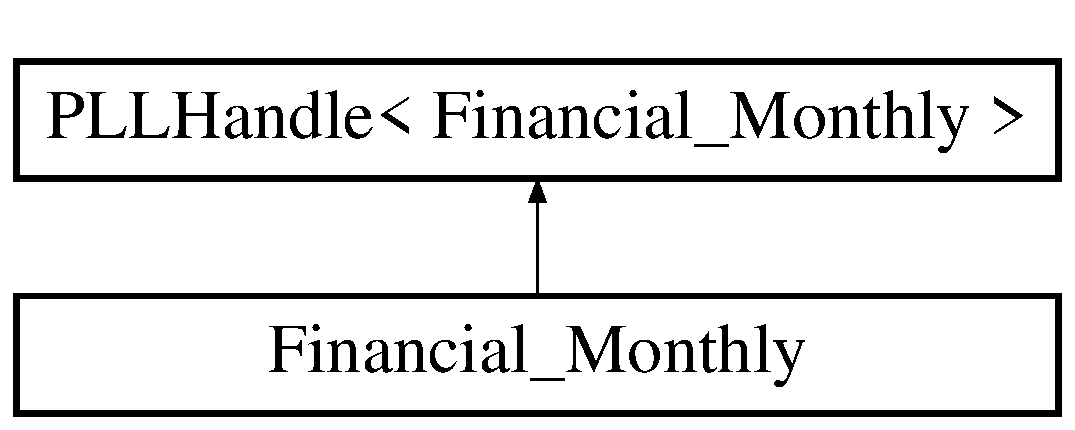
\includegraphics[height=2cm]{classFinancial__Monthly}
\end{center}
\end{figure}
\subsection*{Public Methods}
\begin{CompactItemize}
\item 
{\bf Financial\_\-Monthly} ({\bf String} m)
\item 
{\bf String} {\bf Month} () const
\item 
Financial\_\-Monthly $\ast$ {\bf Find\_\-Month} ({\bf String} m) const
\item 
void {\bf Copy\_\-Categories} (Financial\_\-Monthly $\ast$h)
\item 
void {\bf add} (const {\bf Financial\_\-Note} \&fn)
\end{CompactItemize}
\subsection*{Public Attributes}
\begin{CompactItemize}
\item 
{\bf PLLRoot}$<$ {\bf Financial\_\-Monthly\_\-Category} $>$ {\bf categories}
\end{CompactItemize}
\subsection*{Protected Attributes}
\begin{CompactItemize}
\item 
{\bf String} {\bf month}
\end{CompactItemize}


\subsection{Constructor \& Destructor Documentation}
\index{Financial_Monthly@{Financial\_\-Monthly}!Financial_Monthly@{Financial\_\-Monthly}}
\index{Financial_Monthly@{Financial\_\-Monthly}!Financial_Monthly@{Financial\_\-Monthly}}
\subsubsection{\setlength{\rightskip}{0pt plus 5cm}Financial\_\-Monthly::Financial\_\-Monthly ({\bf String} {\em m})\hspace{0.3cm}{\tt  [inline]}}\label{classFinancial__Monthly_a0}




Definition at line 1136 of file dil2al.hh.



\footnotesize\begin{verbatim}1136 : month(m) {}
\end{verbatim}\normalsize 


\subsection{Member Function Documentation}
\index{Financial_Monthly@{Financial\_\-Monthly}!add@{add}}
\index{add@{add}!Financial_Monthly@{Financial\_\-Monthly}}
\subsubsection{\setlength{\rightskip}{0pt plus 5cm}void Financial\_\-Monthly::add (const {\bf Financial\_\-Note} \& {\em fn})}\label{classFinancial__Monthly_a4}




Definition at line 209 of file finances.cc.

References Financial\_\-Monthly\_\-Category::add(), String::after(), categories, Financial\_\-Note::Expense(), Financial\_\-Monthly\_\-Category::Find\_\-Category(), PLLHandle$<$ Financial\_\-Monthly $>$::head(), PLLRoot$<$ Financial\_\-Monthly\_\-Category $>$::head(), String::index(), PLL\_\-LOOP\_\-FORWARD, String::sub(), PLLRoot$<$ Financial\_\-Monthly\_\-Category $>$::tail(), and Financial\_\-Note::Type().

Referenced by Financial\_\-Monthly\_\-Root::add().



\footnotesize\begin{verbatim}209                                                      {
210   // add by category
211   String cstr = fn.Type();
212   if (cstr.index(BRXidentifier)<0) cstr = "variable";
213   else cstr = cstr.sub(BRXidentifier,0);
214   Financial_Monthly_Category * fc = NULL;
215   if (categories.head()) fc = categories.head()->Find_Category(cstr);
216   if (!fc) { // add category in all months
217     PLL_LOOP_FORWARD(Financial_Monthly,head(),1) {
218       fc = new Financial_Monthly_Category(cstr);
219       e->categories.link_before(fc);
220     }
221     fc = categories.tail(); // retrieve category in this month
222   }
223   // add to category result and by subcategory
224   fc->add(fn.Type().after(','),fn.Expense(),*this);
225 }
\end{verbatim}\normalsize 
\index{Financial_Monthly@{Financial\_\-Monthly}!Copy_Categories@{Copy\_\-Categories}}
\index{Copy_Categories@{Copy\_\-Categories}!Financial_Monthly@{Financial\_\-Monthly}}
\subsubsection{\setlength{\rightskip}{0pt plus 5cm}void Financial\_\-Monthly::Copy\_\-Categories (Financial\_\-Monthly $\ast$ {\em h})}\label{classFinancial__Monthly_a3}




Definition at line 200 of file finances.cc.

References categories, Financial\_\-Monthly\_\-Category::Copy\_\-Sub\-Categories(), PLLRoot$<$ Financial\_\-Monthly\_\-Category $>$::head(), PLLRoot$<$ Financial\_\-Monthly\_\-Category $>$::link\_\-before(), and PLL\_\-LOOP\_\-FORWARD.

Referenced by Financial\_\-Monthly\_\-Root::add().



\footnotesize\begin{verbatim}200                                                              {
201   if (h==this) return; // no other month to copy from
202   PLL_LOOP_FORWARD(Financial_Monthly_Category,h->categories.head(),1) {
203     Financial_Monthly_Category * fc = new Financial_Monthly_Category(e->Category());
204     categories.link_before(fc);
205     fc->Copy_SubCategories(e);
206   }
207 }
\end{verbatim}\normalsize 
\index{Financial_Monthly@{Financial\_\-Monthly}!Find_Month@{Find\_\-Month}}
\index{Find_Month@{Find\_\-Month}!Financial_Monthly@{Financial\_\-Monthly}}
\subsubsection{\setlength{\rightskip}{0pt plus 5cm}Financial\_\-Monthly $\ast$ Financial\_\-Monthly::Find\_\-Month ({\bf String} {\em m}) const}\label{classFinancial__Monthly_a2}




Definition at line 194 of file finances.cc.

References month, and PLLHandle$<$ Financial\_\-Monthly $>$::Next().

Referenced by Financial\_\-Monthly\_\-Root::add().



\footnotesize\begin{verbatim}194                                                                 {
195   if (month==m) return const_cast<Financial_Monthly *>(this);
196   if (Next()) return Next()->Find_Month(m);
197   return NULL;
198 }
\end{verbatim}\normalsize 
\index{Financial_Monthly@{Financial\_\-Monthly}!Month@{Month}}
\index{Month@{Month}!Financial_Monthly@{Financial\_\-Monthly}}
\subsubsection{\setlength{\rightskip}{0pt plus 5cm}{\bf String} Financial\_\-Monthly::Month () const\hspace{0.3cm}{\tt  [inline]}}\label{classFinancial__Monthly_a1}




Definition at line 1138 of file dil2al.hh.



\footnotesize\begin{verbatim}1138 { return month; }
\end{verbatim}\normalsize 


\subsection{Member Data Documentation}
\index{Financial_Monthly@{Financial\_\-Monthly}!categories@{categories}}
\index{categories@{categories}!Financial_Monthly@{Financial\_\-Monthly}}
\subsubsection{\setlength{\rightskip}{0pt plus 5cm}{\bf PLLRoot}$<${\bf Financial\_\-Monthly\_\-Category}$>$ Financial\_\-Monthly::categories}\label{classFinancial__Monthly_m0}




Definition at line 1137 of file dil2al.hh.

Referenced by add(), and Copy\_\-Categories().\index{Financial_Monthly@{Financial\_\-Monthly}!month@{month}}
\index{month@{month}!Financial_Monthly@{Financial\_\-Monthly}}
\subsubsection{\setlength{\rightskip}{0pt plus 5cm}{\bf String} Financial\_\-Monthly::month\hspace{0.3cm}{\tt  [protected]}}\label{classFinancial__Monthly_n0}




Definition at line 1134 of file dil2al.hh.

Referenced by Find\_\-Month().

The documentation for this class was generated from the following files:\begin{CompactItemize}
\item 
{\bf dil2al.hh}\item 
{\bf finances.cc}\end{CompactItemize}
